\documentclass[12pt,a4paper]{article}

\usepackage[T1]{fontenc}
\usepackage[utf8]{inputenc}
\usepackage{amsmath, amssymb}
\usepackage{pgfplots}
\pgfplotsset{compat=1.18}
\usepackage{geometry}
\geometry{margin=2.5cm, top=3cm, bottom=3cm}

\usepackage{xcolor}
\usepackage{tikz}
\usetikzlibrary{shapes.geometric, positioning, calc}
\usepackage{tcolorbox}
\tcbuselibrary{skins, breakable}
\usepackage{fancyhdr}
\usepackage{graphicx}

% --- Configuración de altura de encabezado ---
\setlength{\headheight}{24.64995pt}

% --- Definición de Colores ---
% Aquí definimos los colores principales del documento
% azul: color principal para encabezados, líneas decorativas y énfasis
% azuloscuro: versión oscura del azul para crear contraste visual
% grisosuper: gris oscuro para textos principales y contenido
% grisclaro: gris claro para fondos de cajas de contenido
\definecolor{azul}{RGB}{0, 51, 102}
\definecolor{azuloscuro}{RGB}{0, 40, 80}
\definecolor{grisosuper}{RGB}{51, 63, 72}
\definecolor{grisclaro}{RGB}{240, 242, 245}
\definecolor{verdeescuela}{RGB}{34, 139, 34}

% --- Configuración de Formato ---
% Espaciado entre líneas a 1.5 para mejor legibilidad
\usepackage{setspace}
\onehalfspacing

% --- Estilos de Secciones y Subsecciones ---
\usepackage{titlesec}
% Formato de secciones principales: gris oscuro, tamaño grande, con barra azul debajo
\titleformat{\section}
{\normalfont\fontsize{16}{19}\bfseries\color{grisosuper}}
{\thesection}{1em}{}
[\vspace{0.3em}{\color{azul}\titlerule[2pt]}]

% Formato de subsecciones: azul oscuro, tamaño mediano
\titleformat{\subsection}
{\normalfont\fontsize{14}{17}\bfseries\color{azul}}
{\thesubsection}{1em}{}

% --- Configuración de Encabezado y Pie de Página ---
% Aquí se define el contenido de la parte superior e inferior de cada página
\pagestyle{fancy}
\fancyhf{}
% Encabezado izquierdo: título del documento en azul
\fancyhead[L]{\color{azul}\textbf{Análisis de Consumo de RAM}}
% Encabezado derecho: sección actual en gris
\fancyhead[R]{\color{grisosuper}\textbf{Actividad: Convalidación}}
\fancyfoot[C]{\color{grisosuper}\thepage}
\renewcommand{\headrulewidth}{2pt}
% Línea horizontal azul en el encabezado de cada página
\renewcommand{\headrule}{\hbox to\headwidth{\color{azul}\leaders\hrule height \headrulewidth\hfill}}

% --- Definición de Cajas Personalizadas ---
% Caja para conceptos importantes: fondo gris claro, marco azul
\newtcolorbox{cajaconcepto}{
    colback=grisclaro,
    colframe=azul,
    boxrule=2pt,
    arc=3mm,
    left=5pt,
    right=5pt,
    top=5pt,
    bottom=5pt
}

% Caja para resultados matemáticos: fondo azul claro, marco azul oscuro, título en blanco
\newtcolorbox{cajaresultado}{
    colback=azul!10,
    colframe=azuloscuro,
    boxrule=2.5pt,
    arc=2mm,
    left=8pt,
    right=8pt,
    top=8pt,
    bottom=8pt,
    fonttitle=\bfseries\color{white},
    coltitle=white,
    colbacktitle=azuloscuro,
    title=Resultado
}

\begin{document}

% === PORTADA DEL DOCUMENTO ===
% Aquí se define el diseño visual de la primera página con barras decorativas y logo
\begin{titlepage}
    % Crea un lienzo con elementos decorativos que cubren toda la página
    \begin{tikzpicture}[remember picture, overlay]
        % Barra superior azul (encabezado decorativo)
        \fill[azul] (current page.north west) rectangle ($(current page.north east)+(0,-1.5cm)$);
        % Triángulo gris oscuro en la esquina superior izquierda (efecto visual)
        \fill[grisosuper] ($(current page.north west)+(0,-1.5cm)$) -- 
                          ($(current page.north west)+(4cm,-3cm)$) --
                          ($(current page.north west)+(4cm,-1.5cm)$) -- cycle;
        \fill[azul] (current page.south west) rectangle ($(current page.south east)+(0,1.5cm)$);
        \fill[grisosuper] ($(current page.south west)+(0,1.5cm)$) -- 
                          ($(current page.south west)+(4cm,3cm)$) --
                          ($(current page.south west)+(4cm,1.5cm)$) -- cycle;
        \node at ($(current page.north east)+(-3cm,-3.5cm)$) {\includegraphics[width=5.5cm, height=5.5cm]{LogoUp.png}};
    \end{tikzpicture}
    
    \vspace*{3cm}
    \centering
    \vspace{1.5cm}
    
    {\color{grisosuper}\bfseries\fontsize{20}{24}\selectfont 
    Análisis de Consumo de RAM \\[0.3cm]
    en Servidores Web\\[0.3cm]
    {\fontsize{16}{19}\selectfont (Enfoque en AWS)}\par}
    
    \vspace{0.5cm}
    {\color{azul}\rule{8cm}{2pt}\par}
    
    \vspace{1.5cm}
    {\color{grisosuper}\bfseries\fontsize{16}{19}\selectfont 
    Actividad: Convalidación \par}
    
    \vspace{2cm}
    
    \begin{minipage}{0.8\textwidth}
        \centering
        \begin{tabular}{rl}
            \color{azul}\textbf{Nombre del Alumno:} & \color{grisosuper}Williams Espinosa López \\[0.3cm]
            \color{azul}\textbf{Matrícula:} & \color{grisosuper}251185 \\[0.3cm]
            \color{azul}\textbf{Cuatrimestre y Grupo:} & \color{grisosuper}4° - Grupo "B" \\[0.3cm]
            \color{azul}\textbf{Docente:} & \color{grisosuper}Sirgei García Ballinas \\ [0.3cm]
            \color{azul}\textbf{Asignatura:} & \color{grisosuper}Cálculo Integral \\
        \end{tabular}
    \end{minipage}
    
    \vfill
    
    {\color{grisosuper}\large Jueves, 29 de enero de 2026 \par}
\end{titlepage}

\newpage
\thispagestyle{fancy}
\renewcommand{\contentsname}{\color{grisosuper}Índice}
\tableofcontents
\newpage

\section{Introducción}
% Contexto: por qué estudiamos consumo de RAM en servidores web

Este primer paso desarrolla un análisis del consumo de memoria RAM en un servidor que aloja una página web, con un enfoque particular en servicios de computación en la nube como Amazon Web Services (AWS). El estudio considera una carga constante de 50 usuarios simultáneos y evalúa las fluctuaciones en el uso de recursos debidas a horas pico de acceso.

\begin{cajaconcepto}
% Aquí establecemos claramente qué queremos lograr con este análisis
\textbf{Objetivo:} Modelar matemáticamente el consumo de RAM en función del tiempo y determinar los requerimientos de memoria necesarios para garantizar un servicio estable y eficiente en plataformas de infraestructura en la nube, específicamente AWS EC2.
\end{cajaconcepto}

\vspace{0.5cm}

% Herramientas que usamos y por qué son importantes
El análisis utiliza herramientas de cálculo integral para cuantificar el consumo acumulado de recursos y proporcionar recomendaciones técnicas fundamentadas. Este enfoque es especialmente relevante para la optimización de costos en servicios cloud, donde la asignación eficiente de recursos impacta directamente en los gastos operativos.

\section{Modelado de la Ecuación}
% Esta sección define cómo representamos matemáticamente el consumo de RAM
% Usamos funciones basadas en patrones reales de uso en la región de Chiapas

Para representar el consumo de memoria RAM ($R$) en Gigabytes (GB) respecto al tiempo ($t$) en horas, se desarrolla un modelo matemático dinámico que considera variaciones de tráfico web propias de la región de Chiapas, México (UTC-6), así como un número de usuarios concurrentes superior a 50.

\subsection{Consideración de Horas Pico en Chiapas}
% Aquí identificamos cuándo hay más usuarios usando el sistema
% Es importante para dimensionar recursos correctamente

De acuerdo con patrones de uso web institucional y académico, las horas pico se concentran en los siguientes intervalos:

\begin{itemize}
    \item \textbf{09:00 a 12:00 horas}
    \item \textbf{18:00 a 22:00 horas}
\end{itemize}

Durante estos periodos, el número de usuarios concurrentes y la demanda de recursos incrementan significativamente.

\subsection{Modelo de Usuarios Concurrentes}
% Esta función simula cuántos usuarios están activos en cada hora
% Aumenta durante picos y disminuye en horas bajas

Se define una función continua que modela el número de usuarios activos:

\[
U(t) = 50 + 30\sin\left(\frac{\pi t}{12}\right)
\]

donde:
\begin{itemize}
    \item $U(t)$ es el número de usuarios concurrentes
    \item $t \in [0, 24]$ representa la hora del día
\end{itemize}

\subsection{Modelo de Consumo de Memoria RAM}
% Aquí juntamos todo: carga base + consumo por usuario
% Esto nos da la fórmula final para calcular RAM necesaria

Se consideran los siguientes parámetros:

\begin{itemize}
    \item Carga base del sistema: 2 GB
    \item Consumo promedio por usuario: 0.08 GB (80 MB)
\end{itemize}

La ecuación final del consumo de RAM es:

\begin{cajaresultado}
% Fórmula principal: cantidad fija de RAM + variación según usuarios
\[
R(t) = 6 + 2.4\sin\left(\frac{\pi t}{12}\right)
\]
\end{cajaresultado}

\section{Representación Gráfica del Consumo}
% La gráfica visualiza cómo cambia el consumo de RAM durante el día
% Permite identificar picos y períodos de bajo consumo

\begin{center}
\begin{tikzpicture}
% Configuración general de la gráfica
\begin{axis}[
    title={\color{grisosuper}\textbf{Consumo de RAM en AWS (24 horas)}},
    xlabel={Hora del día},
    ylabel={RAM (GB)},
    xmin=0, xmax=24,
    ymin=2, ymax=9,
    xtick={0,6,9,12,18,22,24},
    grid=both,
    width=13cm,
    height=8cm
]
% Dibuja la curva de consumo usando la función matemática
\addplot [
    domain=0:24,
    samples=200,
    color=azul,
    line width=2pt
]
{6 + 2.4*sin(deg(pi*x/12))};

% Etiqueta que identifica la función graficada
\addlegendentry{$R(t) = 6 + 2.4\sin(\frac{\pi t}{12})$}
\end{axis}
\end{tikzpicture}
\end{center}

\section{Resolución de la Integral}
% Calculamos el consumo TOTAL en un período de 12 horas
% Esto ayuda a entender cuántos recursos se usan en ese lapso

Se calcula el consumo acumulado de memoria RAM durante un periodo de 12 horas:

\[
% Integral que suma todo el RAM usado en 12 horas
\int_{0}^{12} \left( 6 + 2.4\sin\left(\frac{\pi t}{12}\right) \right)\, dt
\]

\subsection{Desarrollo Matemático}
% Separamos la integral en dos partes para resolverla más fácil

Separando la integral:

\[
\int_{0}^{12} 6\, dt + \int_{0}^{12} 2.4\sin\left(\frac{\pi t}{12}\right)\, dt
\]

Primer término:
% Integrar una constante es fácil: cte × variable

\[
\int_{0}^{12} 6\, dt = [6t]_{0}^{12} = 72
\]

Segundo término:
% Para el seno usamos técnica de sustitución

\[
\int 2.4\sin\left(\frac{\pi t}{12}\right) dt
\]

Sea \( u = \frac{\pi t}{12} \Rightarrow du = \frac{\pi}{12} dt \)

\[
= 2.4 \cdot \frac{12}{\pi} \int \sin(u) du
\]

\[
= -\frac{28.8}{\pi}\cos(u)
\]

Evaluando límites:

\[
-\frac{28.8}{\pi}[\cos(\pi) - \cos(0)] = \frac{57.6}{\pi}
\]

\subsection{Resultado Final}
% Aquí combinamos ambos resultados para obtener el consumo total

\begin{cajaresultado}
% El resultado final: RAM total usada en 12 horas
\[
\boxed{
\int_{0}^{12} R(t)\,dt = 72 + \frac{57.6}{\pi}
\approx 90.34\ \text{GB·h}
}
\]
\end{cajaresultado}

\section{Conclusión}
% Resumen de lo aprendido y recomendaciones basadas en el análisis matemático

Con base en el análisis matemático realizado, se establecen las siguientes conclusiones y recomendaciones técnicas para la implementación en AWS:

\begin{cajaconcepto}
% Estos son los requisitos mínimos de RAM que necesitamos
\textbf{Requerimientos de Memoria:}
\begin{itemize}
    \item \textbf{Capacidad mínima recomendada:} 8 GB de RAM
    \item \textbf{Consumo promedio:} 6 GB
    \item \textbf{Pico máximo:} 8.4 GB
    \item \textbf{Margen de seguridad:} 15\% adicional
\end{itemize}
\end{cajaconcepto}

\vspace{0.5cm}

% Explicación de por qué estos números importan en la práctica
El modelo desarrollado demuestra que el consumo de RAM oscila entre 3.6 GB y 8.4 GB durante un ciclo de 24 horas, con una media de 6 GB. Este patrón predecible permite una gestión eficiente de recursos en plataformas como AWS, facilitando decisiones de escalabilidad automática basadas en métricas observables.

El cálculo integral realizado indica que en un período de 12 horas se consume aproximadamente 90.34 GB·h, información crucial para proyectar costos mensuales y seleccionar el tipo de instancia EC2 más adecuado. La función matemática desarrollada proporciona una base sólida para implementar políticas de auto-scaling y optimizar la asignación dinámica de recursos.

\end{document}